\section{Sistemi LTI e trasformata zeta}
La funzione di trasferimento $H(z)$ può essere espressa in termini delle \textbf{radici} dei polinomi al numeratore e al numeratore fattorizzando i due polinomi $N(z)$ e $D(z)$:
$$H(z) = \frac{N(z)}{D(z)} = Kz^{M-N} \frac{(z-c_1)(z-c_2) \dots (z-c_N)}{(z-d_1)(z-d_2)\dots(z-d_N)}$$
La risposta di un sistema LTI viene analizzata attraverso i poli e gli zeri della funzione di trasferimento $H(z)$.

I coefficienti nell'equazione alle differenze corrispondono ai coefficienti nella trasformata, considerando il cambiamento di segno. Al numeratore c'è la parte non ricorsiva, e al denominatore quella ricorsiva. Se non c'è il denominatore, la sequenza è FIR (risposta all'impulso finita).

I sistemi FIR hanno risposta d'impulso limitata, e si può immediatamente passare alla rappresentazione tramite equazione alle differenze dato che i coefficienti sono gli stessi. I sistemi non sono ricorsivi, dato che i FIR possono essere sempre realizzati con sistemi non ricorsivi.

Essi sono in funzione di soli $M$ campioni della sequenza di ingresso, pesati per la risposta all'impulso $h(n)$: dipendono solo da un numero finito di elementi del passato. Dato $h(n)$, si ha subito la trasformata zeta.
$$\{\underset{\Uparrow}1, 2, 0, 4\} \qquad h(n) = \sum_{j=0}^{N-1}\beta_j\delta(n - j) = \delta(n) + 2\delta(n - 1) + 4\delta(n - 3)$$
$$y(n) = \sum_{k=-\infty}^{+\infty} h(k)x(n-k) = \sum_{k=0}^{3}h(k)x(n-k)$$
$$y(n) = x(n) + 2x(n-1) + 4x(n-3) \qquad H(z) = 1+2z^{-1} + 4z^{-3}$$

Studiando i poli si analizza la regione in cui la funzione viene amplificata e cresce in valore, gli zeri dove diminuisce. Insieme quindi danno l'andamento delle frequenze. Un paio di poli complessi e coniugati corrisponde a segnali causali con comportamento a oscillazione.

La frequenza è legata alla \textbf{posizione angolare}, quindi se i poli si trovano nello zero la loro influenza si riflette su tutte le frequenze o nessuna: il contributo è nullo.

Il sistema è \textbf{stabile} se la trasformata di Fourier è interna alla regione di convergenza. 

\begin{figure}[p]
	\centering
	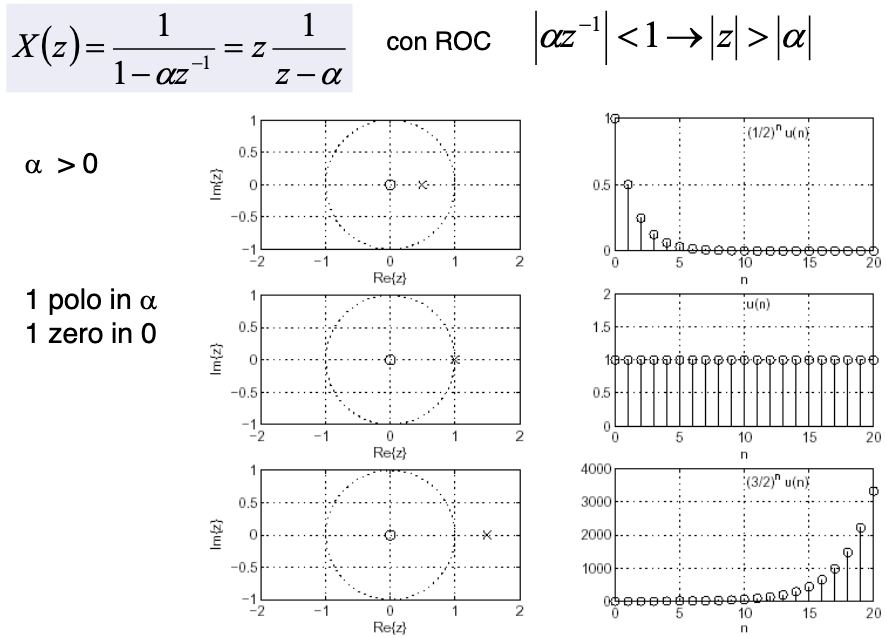
\includegraphics[scale=0.45]{Lezioni/Immagini/rocalpha1} \\
	\vspace{0.5cm}
	\hspace*{0.5cm} 
	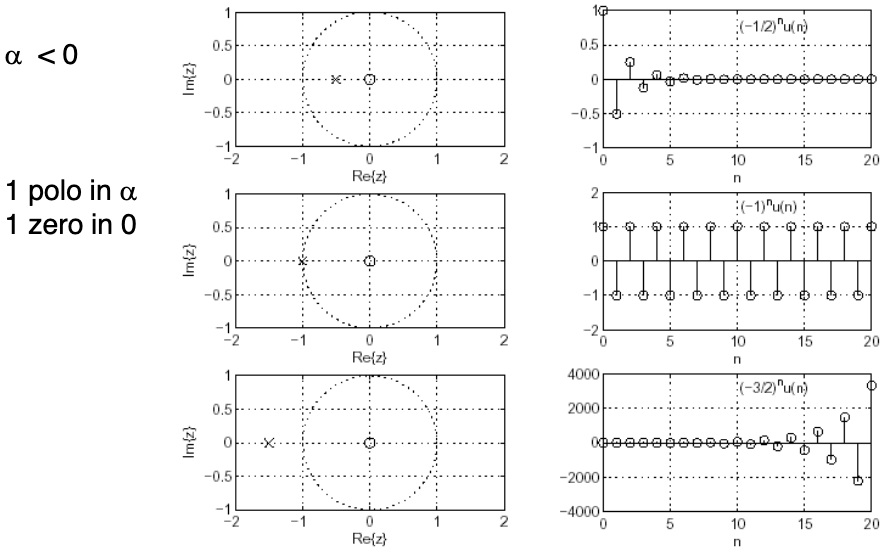
\includegraphics[scale=0.43]{Lezioni/Immagini/rocalpha2}
\end{figure}

\newpage
\subsection{Stabilità BIBO}
La \textbf{stabilità BIBO} di un sistema LTI impone che la risposta all'impulso $h(n)$ sia sommabile in modulo: $\sum_{n=-\infty}^{\infty}\abs{h(n)} < \infty$. Se il sistema è causale, la condizione si traduce nel dominio $z$ imponendo che la funzione di trasferimento $H(z)$ abbia \textit{poli contenuti nella circonferenza di raggio unitario} del piano $z$. 

Le caratteristiche della sequenza dipendono dalla posizione dei poli: la convergenza, e conseguentemente la stabilità, sono determinate dall'appartenenza al cerchio unitario.

I poli all'esterno del cerchio $\abs{z} = 1$ conducono a una risposta all'impulso $h(n)$ con crescita esponenziale, e l'uscita del sistema LTI potrebbe divergere anche in presenza di segnali $x(n)$ d'ingresso costanti. Poli multipli sul cerchio unitario conducono a una crescita di tipo polinomiale.

Poli semplici su $\abs{z} = 1$ possono condurre a una risposta divergente, e dunque a un sistema LTI \textbf{non stabile }secondo la definizione BIBO.

$H(z) = \frac{z}{z-3}$ ha un polo in $z = 3$, infatti ha $h(n) = 3^nu(n)$. \\
$H(z) = \frac{1}{z(z-1)^2}$ ha un polo di ordine 2 in $z = 1$, e risposta all'impulso $h(n) = u(n)$ di tipo rampa, quindi è instabile. \\
$H(z) = \frac{z}{(z-1)}$ ha un polo semplice in $z = 1$, e risposta all'impulso $h(n) = u(n)$ costante (con modulo che tende a infinito).

La circonferenza di raggio unitario dev'essere sempre contenuta nella regione di convergenza per garantire la stabilità del sistema:
\begin{itemize}
	\item Se il sistema è causale, condizione necessaria e sufficiente per la stabilità BIBO è che la funzione di trasferimento $H(z)$ abbia tutti i poli contenuti nella circonferenza di raggio unitario;
	\item Se il sistema è anticausale, condizione necessaria e sufficiente per la stabilità BIBO è che la funzione di trasferimento $H(z)$ abbia tutti i poli all'esterno della circonferenza di raggio unitario, cioè con $\abs{z} > 1$;
	\item Se il sistema è bilatero, condizione necessaria e sufficiente per la stabilità BIBO richiede che la circonferenza di raggio unitario $\abs{z = 1}$ sia contenuta nell'anello circolare che identifica la regione di convergenza ROC nella funzione di trasferimento del sistema.
\end{itemize}

La condizione di stabilità implica che sia sempre possibile identificare la risposta in frequenza $H(e^{j\omega})$, essendo la circonferenza $\abs{z} = 1$ contenuta nella regione di convergenza di $H(z)$.

Un sistema LTI fisicamente realizzabile deve possedere una risposta all'impulso $h(n)$ \textbf{causale} e con \textbf{coefficienti reali}. Ciò significa che:
\begin{enumerate}
	\item La regione di convergenza $H(z)$ corrisponde all'esterno di un cerchio di raggio minore del polo di $H(z)$ di valore assoluto massimo (causalità);
	\item Per ogni polo e zero complesso, deve essere presente anche il rispettivo complesso coniugato. Poli e zeri sull'asse reale possono essere singoli: hanno parte immaginaria nulla, quindi coincidono con i propri complessi coniugati (coefficienti reali).
\end{enumerate}

Quando il polinomio è espresso tramite potenze negative, una costante corrisponde all'assenza di ritardo, quindi sia al numeratore che al denominatore si somma 1 per indicare l'istante corrente. Tutte le volte che la soluzione non è a coefficienti reali, è presente il complesso coniugato. I monomi vengono espressi in termini di potenze negative di $z$.

\section{Filtri con poli e zeri}
Avendo a disposizione la trasformata con i poli e gli zeri, conoscendo le proprietà di continuità della funzione analitica è possibile conoscere l'andamento delle frequenze.

Se un polo reale è molto vicino al cerchio di raggio unitario, si ha che il denominatore si annulla con valori prossimi a $\rho = 1$, ma a $z = 1$ c'è un picco e la risposta cresce in funzione alla posizione del polo. In altre parole, ogni polo ha un'influenza sulle frequenze a seconda della loro vicinanza.

I \textbf{poli} devono essere posizionati in prossimità del cerchio di raggio unitario nelle pulsazioni complesse $z$ corrispondenti alle componenti armoniche nel segnale d'ingresso $x(n)$ che devono essere \textbf{enfatizzate}.

Gli \textbf{zeri} devono essere posizionati vicino ai punti $z$ del cerchio di raggio unitario corrispondenti alle componenti armoniche del segnale d'ingresso $x(n)$ che devono essere \textbf{attenuate}.

Per la stabilità e la realizzabilità fisica (causalità), tutti i poli del filtro devono cadere nella circonferenza di raggio unitario, mentre gli zeri possono essere posizionati in qualunque punto del piano. Entrambi devono essere presenti a coppie complesse e coniugate.

Introducendo un fattore di normalizzazione $1 - \alpha$, è possibile confrontare i filtri con valore di picco (guadagno) unitario. Se la frequenza è causale, il numero di zeri non deve superare il numero di poli.

\begin{figure}[h]
	\centering
	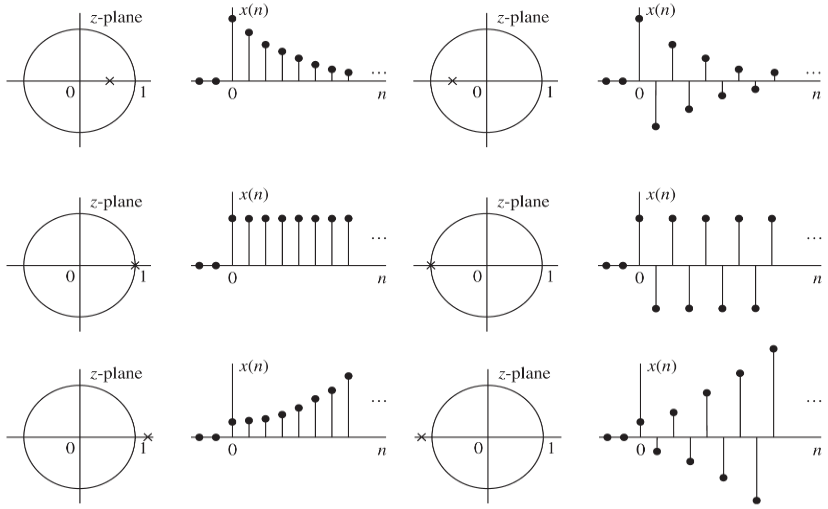
\includegraphics[scale=0.45]{Lezioni/Immagini/polizeri1}
\end{figure}
\begin{figure}[h]
	\centering
	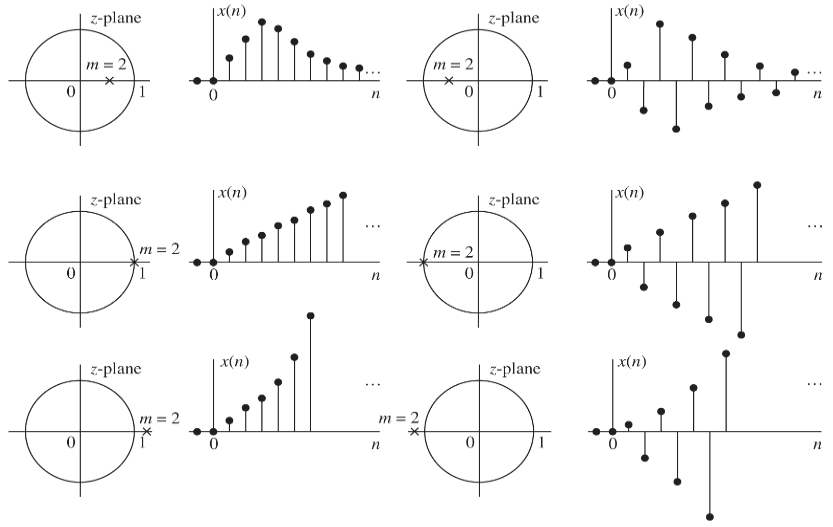
\includegraphics[scale=0.45]{Lezioni/Immagini/polizeri2}
	\vspace{0.5cm}
	\hspace*{0.5cm} 
\end{figure}

\newpage
Ricostruendo la frequenza a partire dal filtro, si ha $H(z) = k \frac{z}{z - \alpha} = \frac{k}{1 - \alpha z^{-1}}$ con $k$ costante. Se il guadagno è unitario, $\abs{H(z)_{f=0 \land z=1}} = 1$ da cui $k = 1 - \alpha$ (filtro con sempre la stessa altezza).

Solitamente la massima oscillazione $\delta_2$ permessa in banda proibita viene espressa in dB attraverso l'oscillazione $R-P$, dove $R_p = -10\log(\delta_2^2)$. 

La banda proibita è data dall'insieme delle frequenze per le quali il guadagno è inferiore a un'opportuna soglia di attenzione, che normalmente viene stabilita in funzione dell'applicazione. Indicando con $v_s$ la frequenza di stop e con $v_c$ la frequenza di taglio, le frequenze comprese tra esse costituiscono la banda di transizione.

\subsection{Passa-basso e passa-alto}
Tanto più i poli sono vicini all'asse reale, più influenzano le frequenze basse (filtro passa-basso).
 
 I poli del filtro devono essere posizionati nelle pulsazioni complesse $z$ corrispondenti alle frequenze della banda passante di $H(e^{j\omega})$: $\abs{\omega} \in [\omega_t, \pi]$.
 
 Gli zeri devono essere posizionati in prossimità, oppure sul cerchio $\abs{z} = 1$ nelle pulsazioni complesse $z$ corrispondenti alle frequenze $\abs{\omega} \in [\omega_t, \pi]$.
 
Lo zero nell'origine $z = 0$ non ha alcun effetto sulla frequenza, essendo distante dalla circonferenza di raggio unitario: in questo caso la risposta in frequenza è determinata dalla posizione del polo.

Lo zero in $z = -1$, al contrario, enfatizza l'attenuazione alle alte frequenze. Essendo sulla circonferenza di raggio unitario, esso compare anche sulla risposta in frequenza del filtro in corrispondenza delle frequenze numeriche $\pm \nicefrac{1}{2}$.

\begin{figure}[h]
	\centering
	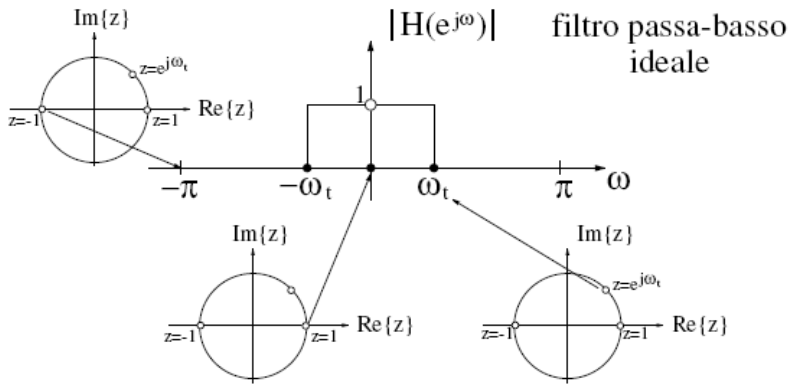
\includegraphics[scale=0.4]{Lezioni/Immagini/passabasso}
\end{figure}

Per enfatizzare le basse frequenze, è sufficiente inserire degli zeri per farle crescere di valore. Creando monomi con radici e aggiungendole al numeratore e al denominatore, si creano filtri in grado di alzare o abbassare le frequenze manipolando le posizioni di poli e zeri. Il numero di zeri non può essere superiore al numero di poli.

Nella realtà bisogna considerare che è impossibile azzerare completamente una parte di frequenza, ma ci saranno delle oscillazioni più o meno ampie.

Per realizzare un filtro passa-banda, è sufficiente unire un passa-basso e un passa-alto, per esempio posizionando due zeri in $z = 1$ e $z = -1$ con i rispettivi poli complessi e coniugati in $z = \rho e^{\pm j\pi/2}$ con $\rho < 1$.

\subsection{Sistema inverso}
Un \textbf{sistema inverso} ha lo scopo di compensare i poli e gli zeri, ed è un sistema che inverte il comportamento di un altro sistema LTI tale che la risposta rimanga inalterata.

Esempio: durante la trasmissione di dati attraverso il canale telefonico, il mezzo distorce il segnale trasmesso ottenendo in uscita un segnale $y(n) \neq x(n)$.

La compensazione della distorsione subita da $x(n)$ avviene in due fasi:
\begin{enumerate}
	\item Stima della risposta in frequenza $H(e^{j\omega})$ del mezzo di trasmissione;
	\item Filtraggio del segnale ricevuto $y(n)$ con un equalizzatore, sistema LTI che ha come risposta in frequenza la funzione $H^{-1}(e^{j\omega})$.
\end{enumerate}

Se la stima del canale è condotta in modo ideale, si riesce a compensare perfettamente la distorsione introdotta dal mezzo di trasmissione.

La cascata di un sistema e del suo inverso ha una funzione di trasferimento pari a una costante unitaria nel piano $z$ (il numeratore di uno dev'essere uguale al denominatore dell'altro e viceversa), definita sistema identità:
$$H_C(z) = H(z)H_I(z) = H(z)H^{-1}(z) = 1$$
Una classe di sistemi che ammettono l'inverso è quella dei sistemi caratterizzati da una trasformata z razionale.

La funzione di trasferimento del sistema inverso possiede zeri corrispondenti ai poli, e poli corrispondenti agli zeri del sistema diretto.

I sistemi LTI fisicamente realizzabili devono essere causali, con regione di convergenza in $\abs{z} >$ polo di valore assoluto maggiore. Per un sistema stabile, il modulo dei poli dev'essere $\abs{z_p} < 1$.

Se un sistema LTI con poli e zeri nel cerchio di raggio unitario rispetta queste condizioni, esso ammette un sistema inverso causale e stabile.

\subsection{Sistemi passa-tutto}
Questi filtri non modificano le frequenze del segnale, ma effettuano altre operazioni (ritardo, anticipo), e dev'esserci una precisa relazione tra i poli e gli zeri. La risposta all'impulso è sempre \textbf{costante}, per ogni frequenza: $H(e^{j\omega}) = 1$.

I coefficienti del polinomio al numeratore sono in ordine inverso rispetto a quelli del denominatore, e ciò viene garantito imponendo il modulo quadro unitario. Raccogliendo $z$, il numeratore resta invariato e il denominatore viene invertito. 

Un polo, quindi, è il reciproco di uno zero (e viceversa):
\begin{itemize}
	\item Se $p_k$ è un polo di $H(z)$, allora $\frac{1}{p_k}$ è uno zero;
	\item Per la realizzabilità fisica, se $p_k$ è un polo complesso dovrà essere polo anche $p_k*$;
	\item Di conseguenza, $\frac{1}{p_k}$ è uno zero.
\end{itemize}

Se uno è all'interno della circonferenza, l'altro è fuori: un sistema LTI passa-tutto causale e stabile presenta poli nel cerchio di raggio unitario nl piano $z$, e zeri all'esterno del cerchio $\abs{z} = 1$. Di conseguenza, un sistema LTI passa-tutto stabile non ammette sistema inverso stabile.

\begin{figure}[h]
	\centering
	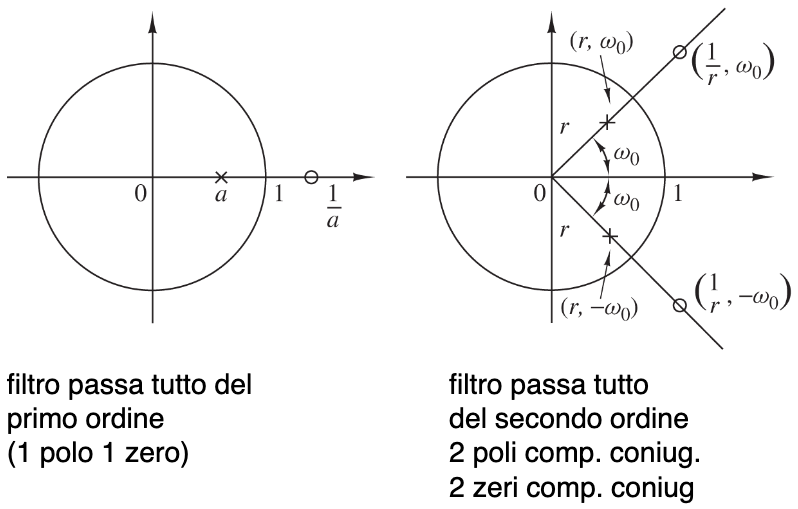
\includegraphics[scale=0.4]{Lezioni/Immagini/passatutto}
\end{figure}


